% Раздзел 1 — метадалогія devops
\section{Метадалогія Devops}

\subsection{Паняцце Devops}

Паняцце Devops не мае агульнапрынятага азначэння.
Азначэнне Devops змяняецца ў залежнасці ад часу, метадаў укаранення,
пастаўленых мэт унутры кампаніі.
У табліцы \ref{table:Definition of Devops} прыведзены некаторыя
азначэнні, каторыя сустракаюцца ў літаратуры.

\begin{table}[htbp]
    \caption{Варыянты азначэнняў Devops}
    \begin{tabular}{|p{0.70\textwidth}|p{0.24\textwidth}|} 
        \hline
        \textbf{Азначэнне Devops}
        &
        \textbf{Сэнс азначэння}  \\ 
        \hline
        Devops -- гэта набор практык, які прызначыны для
        памяншэння часу паміж прыняццямі змен ў сістэме і
        ўнясення іх ў працэс вытворчасці з гарантыяй
        высокай якасці\ref{book:DevOps: A Software Architect's Perspective}
        &
        Арыентацыя на дасягненне мэты (хуткая дастаўка
        якаснага праграмнага забеспячэння) \\ 
        \hline
        Devops -- гэта культурны рух, які змяняе адносіны людзей
        да працы і да яе вынікаў\ref{book:Effective Devops}
        & Арыентацыя на супрацоўніцтва \\ 
        \hline
        Devops -- камбінацыя культуры, практык і інструментаў,
        каторая павялічвае здольнасць арганізацыі
        пастаўляць праграмы і сервісы
        з высокай хуткасцю: развіццё і паляпшэнне прадукцыі
        ў больш хуткім тэмпе,
        чым арганізацыі, якія карыстаюцца традыцыйным спосабам распрацоўкі
        праграмнага забеспячэння і
        кіравання працэсамі інфраструктуры.\ref{site:aws.amazon.com/devops}
        & Арыентацыя на супрацоўніцтва і дасягненне мэты
        (паскарэнне тэмпаў развіцця прадукту) \\
        \hline
        Devops -- набор практык, накіраваны на актыўнае ўзаемадзеянне
        спецыялістаў па распрацоўцы і
        спецыялістаў па інфармацыйна-тэхналагічнаму
        абслугоўванню і ўзаемную інтэграцыю
        іх працоўных працэсаў
        адно ў другое\ref{site:ru.wikipedia.org/wiki/devops}
        &
        Арыентацыя на супрацоўніцтва \\
        \hline
    \end{tabular}
    \label{table:Definition of Devops}
\end{table}

З табліцы \ref{table:Definition of Devops} можам заключыць,
што паняцце Devops уключае ў сябе як культурны, так і
тэхнічны складнікі.
Пры гэтым набор інструментаў, такіх як Chef альбо Docker,
з'яўляецца складнікам Devops дзякуючы спосабам іх прымянення,
а не ў сілу характарыстык саміх інструментаў.\ref{book:Effective Devops}
Такім чынам неабходна адзначыць, што ў першую чаргу Devops разглядаецца
як змяненне культуры арганізацыі,
а іменна адносін паміж камандамі (у прыватнасці каманды распрацоўшчыкаў і
каманды тэхнічнага абслугоўвання).

\subsection{Мадэль CALMS}

Нягледзячы на разнастайнае тлумачэнне тэрміна, Devops мае
пэўныя агульнапрызнаныя элементы.
Гэтыя элементы складаюць мадэль CALMS\ref{article:Challenges in Adopting a Devops} (малюнак \ref{fig:CALMS model}):
\begin{enumerate}
    \item Culture (культура),
    \item Automation (аўтаматызацыя),
    \item Lean (ашчаднасць),
    \item Measurement (мера),
    \item Sharing (абмен).
\end{enumerate}

\begin{figure}[h!]
    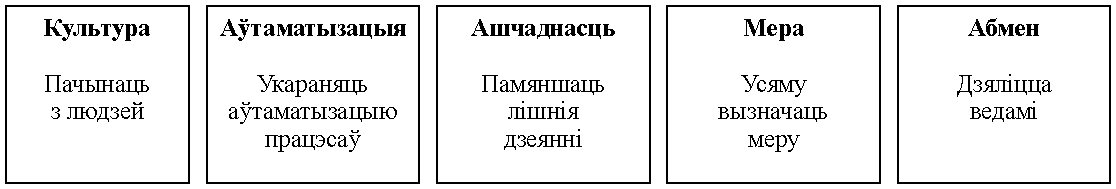
\includegraphics[width=\linewidth]{CALMS.pdf}
    \caption{Мадэль CALMS}
    \label{fig:CALMS model}
\end{figure}

\vspace{-\baselineskip}
\subsubsection{Kyльтура.}

Галоўная ідэя Devops -- змяніць закрытую культуру арганізацыі
на адкрыты спосаб супрацоўніцтва паміж камандамі.
Уцягнуць персанал тэхнічнай эксплуатацыі ў працэсы
распрацоўкі праграм. Акрамя таго, забяспечыць іх уклад на
сходзе для планавання, агляду праектаў, каб яны мелі магчымасць
выказаць уласныя ідэі ўжо на ранніх стадыях працэсу
распрацоўкі.
Humble і Molesky (2011 год) заўважылі, што ўзаемадзеянне з ка\-ман\-дамі
тэхнічнай эксплуатацыі неабходна для каманд распрацоўшчыкаў.
Абодва бакі павінны ў аднолькавай меры ўдзельнічаць у аналізе знаходжання
першапрычын ў выпадку вытворчых інцыдэнтаў, у знаходжанні спосабаў
развязвання праблемы як на этапах распрацоўкі, так і дастаўкі прадукту кліенту.

%Без разумення працэсаў, каторыя адбываюцца ўнутры іншых каманд
%(тэхнічнай эксплуатацыі, тэсціравання), немагчыма дабіцца
%%палітыкі неабвінавачвання ў кампаніі.
%Палітыка неабвінавачвання прадугледжвае прызнанне чалавечых памылак і
%разглядае іх у якасці магчымасці палепшыць прадукцыйнасць кампаніі
%пры дапамозе аналізу першапрычын і наступнага недапушчэння
%аналагічных памылак.
%Калі супрацоўнікі кампаніі не баяцца быць абвінавачанымі і
%пакаранымі за памылкі, адкрываецца шлях да новых інавацый,
%павялічваецца матывацыя і адданасць кампаніі.
%
%У асяроддзі супрацоўніцтва знікае такая праблема, як перакладванне
%адказнасці на іншыя каманды, дазваляе на ранніх стадыях знаходзіць
%праблемы ў праграмных прадуктах або паслугах.

\subsubsection{Аўтаматызацыя.}

%
%З вышэй прыведзеных азначэнняў тэрміна Devops можам вызначыць,
%што, хаця не існуе адзінага разумення метадалогіі Devops,
%у кожным выпадку значная ўвага надаецца культуры ўнутры арганізацыі,
%узаемадзеянню спецыялістаў паміж сабой.
%Дадзеная асаблівасць тлума\-чыц\-ца тым, што метадалогія Devops сфармавалася
%на аснове гібкіх метадалогій, у якіх адбываецца пераход фокуса на
%асобных людзей, узаемадзеянне і супрацоўніцтва.
%
%%Аднак рух Devops пашырае прынцыпы гібкай распрацоўкі праграм
%і прымяняе іх на ўзроўні арганізацыі ў цэлым,
%у той час як іншыя гібкія метадалогіі акцэнтавалі ўвагу толькі на
%распрацоўшчыках праграм.
%
%Нягледзячы на разнастайнае тлумачэнне тэрміна, Devops мае пэўныя
%культурныя прын\-цы\-пы. Гэтыя прынцыпы складаюць мадэль CALMS:
%Culture (культура), Automation (аўтаматызацыя),
%Lean (беражлівасць), Measurement (мера), Sharing (абмен).%
%\ref{article_challenges_in_adopting_a_Devops}
%
%Мадэль CALMS прадстаўлена на малюнку \ref{fig:CALMS model}.
%
%\begin{figure}[h!]
%    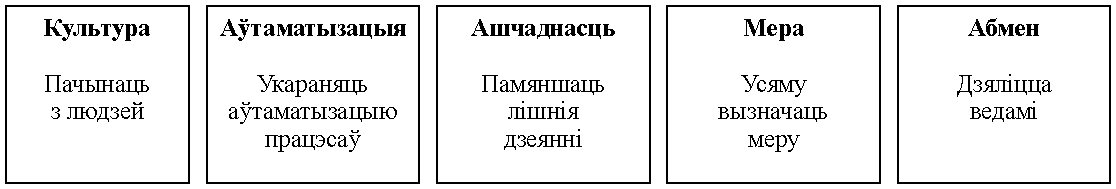
\includegraphics[width=\linewidth]{CALMS.pdf}
%    \caption{мадэль CALMS}
%    \label{fig:CALMS model}
%\end{figure}
%
%\vspace{-\baselineskip}
%\subsubsection{Мадэль CALMS -- культура.}
%
%Прыняцце метадалогіі Devops пачалося з культуры.
%У той час як матэрыяльная частка Devops змяшчае новыя працэсы і
%інструменты для бесперапыннай дастаўкі і інтэграцыі,
%Devops, усяго толькі, папулярнае слова,
%калі "культура арганізацыі" не ахоплівае ўсе рэчы,
%што ідуць у камплекце (Wilsenach 2015).
%
%Галоўная ідэя Devops -- змяніць культуру арганізацыі з
%закрытых скрынь (асобныя ка\-ман\-ды) на адкрыты спосаб супрацоўніцтва
%паміж імі.
%Уцягнуць персанал тэхнічнай эксплуатацыі ў працэсы
%распрацоўкі праграм. Акрамя таго, неабходна іх прысутнасць на
%сходзе для планавання, агляду праектных каманд, каб яны маглі
%падзяліцца ўласнымі ідэямі і ведамі ўжо на ранніх стадыях працэсу
%распрацоўкі.
%Humble і Molesky (2011 год) заўважылі, што абмен з ка\-ман\-дамі
%тэхнічнай эксплуатацыі неабходны для распрацоўшчыкаў, і яны
%павінны ў аднолькавай меры ўдзельнічаць у аналізе знаходжання
%першапрычын ў выпадку вытворчых інцыдэнтаў.
%
%Без разумення працэсаў, каторыя адбываюцца ўнутры іншых каманд
%(тэхнічнай эксплуатацыі, тэсціравання), немагчыма дабіцца
%палітыкі неабвінавачвання ў кампаніі.
%Палітыка неабвінавачвання прадугледжвае прызнанне чалавечых памылак і
%разглядае іх у якасці магчымасці палепшыць прадукцыйнасць кампаніі
%%пры дапамозе аналізу першапрычын і наступнага недапушчэння
%аналагічных памылак.
%Калі супрацоўнікі кампаніі не баяцца быць абвінавачанымі і
%пакаранымі за памылкі, адкрываецца шлях да новых інавацый,
%павялічваецца матывацыя і адданасць кампаніі.
%
%У асяроддзі супрацоўніцтва знікае такая праблема, як перакладванне
%адказнасці на іншыя каманды, дазваляе на ранніх стадыях знаходзіць
%праблемы ў праграмных прадуктах або паслугах.
%
%\subsubsection{Мадэль CALMS -- аўтаматызацыя.}
